\chapter{Detalji implementacije, treniranja i testiranja}
\label{ch:implementacija}

U ovoj glavi opisani su izvršeni eksperimenti, kao i struktura koda. Implementacija i testiranje zasnovani su na radovima \cite{dqn_mnih} i \cite{dqn_dm}.
\section{Detalji implementacije}
\label{sec:implementacija}
Prilikom implementacije, korišćen je programski jezik python\cite{python}, verzija $3.5.2$ kao i sledeće biblioteke:
\begin{itemize}
	\item \texttt{NumPy}\cite{numpy} -- Biblioteka otvorenog koda za numeričko izračunavanje. Korišćena je verzija $1.14.1$.
	%	1.14.1
	% http://www.numpy.org/ 
	\item \texttt{Keras}\cite{keras} -- Biblioteka otvorenog koda koja pruža visoko apstraktni API, što je čini jednostavnim za korišćenje. Ova biblioteka zahteva pozadinski endžin za izračunavanje; u ovu svrhu je korišćena biblioteka \texttt{TensorFlow}\cite{tensorflow}. Verzija biblioteke \texttt{Keras} koja je upotrebljavana je $2.2.0$, dok je verzija biblioteke \texttt{TensorFlow} $1.5.0$.
	%	2.2.0
	% https://keras.io/
	\item  \texttt{OpenAI~Gym}\cite{openai_gym} -- Biblioteka otvorenog koda koja pruža mogućnost korišćenja već gotovih okruženja radi istraživanja raznih pristupa učenju potkrepljivanjem. Korišćena je verzija $0.10.5$ ove biblioteke.
	%	0.10.5
	% https://gym.openai.com/
\end{itemize}
% PYTHON: 3.5.2
% KERAS: 2.2.0
% OPENAI GYM: 0.10.5
% TENSORFLOW: 1.5.0
% NUMPY: 1.14.1
Implicitno su korišćene i biblioteke od kojih navedene biblioteke zavise. U sklopu implementacije korišćeni su i neki moduli koji su deo standardne biblioteke jezika python.
\par 
Implementacija $DQN$ sastoji se iz dve klase, {\em DRLAgent} i {\em ExperienceReplay}, i nekoliko pomoćnih funkcija. Struktura koda opisana je u nastavku, na apstraktnom nivou. Ovo znači da su opisi nekih funkcija, koje nisu od važnosti za shvatanje koda, izostavljeni. Izvorni kod može se naći na sledećoj adresi: \url{https://github.com/NikolaMilev/DeepRL}. \textcolor{red}{Napravi novi repo i refaktorisi pa onda izmeni tekst ovde ako treba}.
\par 
Klasa \texttt{DRLAgent} opisuje funkcionisanje agenta koji se obučava prateći $DQN$ algoritam. Glavne komponente klase su memorija i $Q$ i ciljna mreža. Metodi bitni za učenje su:
\begin{itemize}
	\item \texttt{chooseAction(self, state)}\footnote{Pri pisanju instancnih metoda u jeziku python, prvi argument je uvek referenca na objekat nad kojim se taj metod poziva. Ta referenca označava se ključnom reči \texttt{self}} -- Vrši odabir akcije na osnovu stanja koje je prosleđeno referencom \texttt{state}. Odabir se vrši u skladu sa $\varepsilon$-pohlepnom politikom.
	\item \texttt{trainOnBatch(self, batchSize)} -- Trenira $Q$ mrežu nasumičnim uzorkovanjem memorije, koristeći formule opisane u algoritmu \ref{alg:dqn}.
	\item \texttt{test(self, network, numSteps)}\footnote{Parametar \texttt{network} stoji jer je isti kod korišćen za obučavanje raznih varijacija algoritma pri ispitivanju njegovih komponenti.} -- Vrši testiranje ciljne mreže u skladu sa pravilima opisanim u delu \ref{sec:testiranje}. Testiranje traje \texttt{numSteps} koraka.
	\item \texttt{learn(self, numEpisodes)} -- \textcolor{red}{[OBRISI NUMEPISODES?]} Vrši obučavanje agenta. 
\end{itemize}
\par 
Klasa \texttt{ExperienceReplay} opisuje omotač oko instance klase \texttt{deque}, koja opisuje objedinjenje pojmova steka i reda.\footnote{Dokumentacija ove klase može se naći na adresi \url{https://docs.python.org/3/library/collections.html\#collections.deque}.} Bitni metodi klase su:
\begin{itemize}
	\item \texttt{addTuple(self, state, action, reward, nextState, terminal)} -- Dodaje petorku \texttt{state, action, reward, nextState, terminal)} u memoriju. Prva četiri elementa odgovaraju četvorki $(s, a, r, s')$, odnosno jednom prelazu koji je agent video, dok peti element predstavlja istinitosnu vrednost koja označava da li je stanje $s'$ završno. Ovu informaciju neophodno je čuvati jer se u samim stanjima ona ne nalazi.
	\item \texttt{getMiniBatch(self, sampleSize)} -- Dohvata uzorak veličine \texttt{sampleSize} iz memorije.
\end{itemize}
\par 
Pored opisanih klasa, kod sadrži i funkcije koje pomažu boljoj strukturi koda:
\begin{itemize}
	\item \texttt{buildNetwork(height, width, depth, numActions)} -- Koristeći pozive iz biblioteke Keras, gradi neuronsku mrežu i vraća referencu na dati objekat.
	\item \texttt{copyModelWeights(srcModel, dstModel)} -- Kopira težine mreže \texttt{srcModel} u mrežu \texttt{dstModel}.
	\item \texttt{saveModelWeights(model, name)} -- Čuva neuronsku mrežu na putanju određenu argumentom \texttt{name}.
	\item \texttt{preprocessSingleFrame(img)} -- Vrši pretprocesiranje jedne slike sa ekrana, opisano u \ref{ss:pretprocesiranje}.
	\item \texttt{transformReward(reward)} -- Transformiše nagradu.
\end{itemize}
\par 
U više navrata je rečeno da $DQN$ algoritam uči nad slikama ekrana i nagradom dobijenom od okruženja. Međutim, jedna slika ne daje mnogo informacija. Na primeru igre Breakout, ukoliko je dostupna samo jedna slika ekrana, nemoguće je odrediti u kom se pravcu kreće loptica, ni kojom brzinom. Isto važi i za pločicu koja služi za odbijanje loptice. Međutim, iz nekoliko uzastopnih slika može se odrediti smer i brzina kretanja loptice i pločice. Na slici \ref{fig:ss} prikazane su četiri uzastopne slike sa ekrana.\footnote{Radi ilustracije, nisu prikazane uzastopne slike već je razlika između njih 7 slika. Prikazivanje uzastopnih slika sa ekrana dalo bi kao rezultat 4 skoro identične slike.} 

\begin{figure}
	\centering
	\resizebox{.24\linewidth}{!}{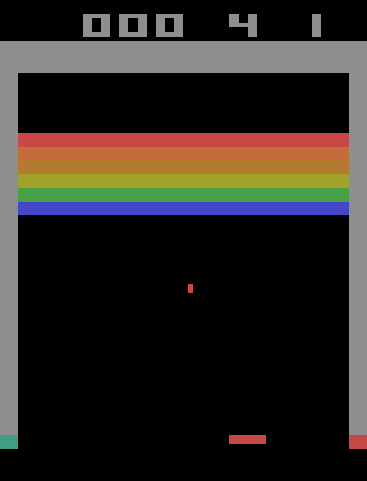
\includegraphics{img/screenshots/1}}
	\resizebox{.24\linewidth}{!}{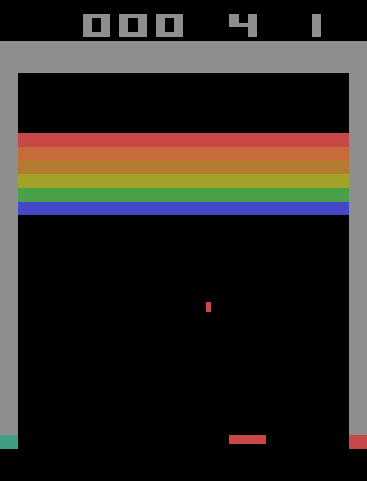
\includegraphics{img/screenshots/2}}
	\resizebox{.24\linewidth}{!}{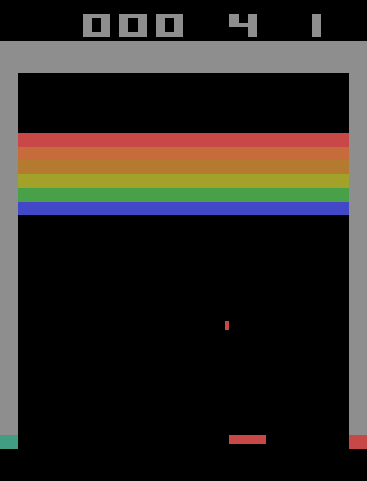
\includegraphics{img/screenshots/3}}
	\resizebox{.24\linewidth}{!}{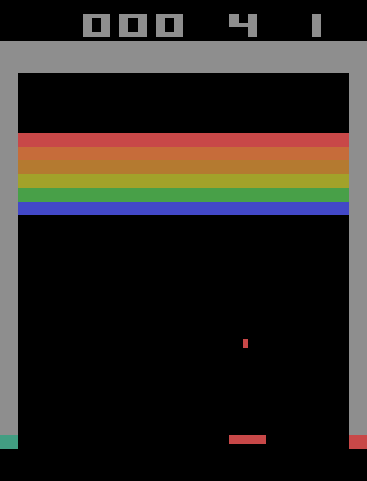
\includegraphics{img/screenshots/4}}
	\caption{Prikaz 4 uzastopna stanja ekrana u igri Breakout. Pločica miruje dok se loptica kreće ka donjem desnom uglu ekrana.}
	\label{fig:ss}
\end{figure}
\par 
Kako igre sa Atari 2600 konzole prikazuju $60$ slika u sekundi (eng.~{\em frame per second},~skr.~{\em fps}) i kako nije realno delati tom frekvencijom, vrši se preskakanje slika (eng.~{\em frame skipping}). Biblioteka \texttt{OpenAI Gym} pruža mogućnost korišćenja raznih vrednosti za broj preskočenih slika. U ovom radu, koristi se okruženje pod imenom \texttt{BreakoutDeterministic-v4}, što znači da će okruženje za jedan poziv kojim se vrši akcija izvršiti tu akciju na $4$ uzastopne slike koja se prikazuje. Deo imena \texttt{Deterministic} označava da će se uvek pozivom prikazivati svako četvrto stanje ekrana; neka okruženja dopuštaju da se preskakanje vrši nasumično, u nekom intervalu dozvoljenih vrednosti. Na primer, okruženje \texttt{Breakout-v0} za svaki poziv vrši preskakanje nasumično odabranog broja slika iz intervala $[1,4]$. \textcolor{red}{RUZNO, PREFORMULISI} U ovoj implementaciji, po uzoru na rad \cite{dqn_dm}, agent će videti svako četvrto stanje ekrana. 

\subsection{Pretprocesiranje}
\label{ss:pretprocesiranje}
Okruženja koja služe kao omotači oko igara sa konzole Atari 2600 u \texttt{OpenAI Gym} biblioteci kao stanje ekrana vraćaju RGB slike dimenzija $210 \times 160$ zapisane u \texttt{NumPy} nizu. Na te slike primenjuje se pretprocesiranje u cilju smanjenja računskih zahteva modela. To pretprocesiranje podrazumeva tranformaciju slike tako da se svaki piksel, koji je trojka koja određuje količinu crvene ($R$), plave ($B$) i zelene ($G$) boje zameni njegovom osvetljenošću ($Y$), određenom na sledeći način:
\begin{equation}
\label{eq:lum}
	Y = 0.299 R + 0.587 G + 0.114 B
\end{equation}
Kako su sve vrednosti $R$, $G$ i $B$ u intervalu $[0, 255]$ i kako se koeficijenti sabiraju na $1$, novodobijena vrednost je u intervalu $[0, 255]$. Vrednosti svakog piksela se u ulaznom sloju mreže dele sa $255$ i time dovode na interval $[0, 1]$. Još jedna transformacija koja se primenjuje na slike je njihovo smanjivanje. U radu \cite{dqn_dm} predloženo je da se slike skaliraju na dimenzije $84 \times 84$ ali, radi jednostavnosti implementacije i brzine izvršavanja, odlučeno je da će se u ovoj implementaciji visina i širina slike prepolove.

\subsection{Prelazi i čuvanje u memoriji}

U cilju čuvanja informacija o smeru kretanja objekata na ekranu, svako stanje biće sačinjeno od određenog broja uzastopnih stanja koja agent vidi. Svaki prelaz sačuvan u memoriju u stvari je petorka oblika $(s, a, r, s', t)$. 
Ono na šta pri implementaciji treba obratiti pažnju su memorijski zahtevi. Nakon transformacije, dobijene slike su dimenzija $105 \times 80$ i njihove koordinate implicitno su zapisane u pokretnom zarezu. Ukoliko je jednostruka tačnost u pitanju, jedno stanje zauzima $32.8125~kB$. Dakle, čuvanje milion stanja, kako je predloženo u radu \cite{dqn_dm}, zahteva između $32$ i $33~GB$ memorije. Ovo je moguće popraviti. Naime, kako su vrednosti dobijene nakon transformacije u intervalu $[0, 255]$ i kako će kasnije biti transformisane tako da staju u interval $[0, 1]$, to je bez gubitka značajne količine podataka moguće zaokružiti ih i čuvati ih u jednobajtnom podatku. Biblioteka \texttt{NumPy} definiše tip \texttt{uint8} koji ovo omogućuje. Takođe treba paziti na to da uzastopna stanja dele sve sem jedne slike. Ukoliko se stanja definišu tako da sadrže reference na pojedinačne slike umesto pravljenja novog niza, deljenje referenci osigurava da se neće praviti bespotrebne kopije podataka. Zajedno sa ostalim memorijskim zahtevima, prilikom treniranja agenta bilo je zauzeto oko {\em 10~GB} memorije.

\section{Detalji treniranja}
\label{sec:treniranje}
U ovom delu opisana je arhitektura mreže, kao i ostali bitni metaparametri. Zbog hardverskih ograničenja, eksperimentisano je samo sa igrom Breakout sa Atari 2600 konzole. Zbog nedovoljno objašnjene implementacije u radu \cite{dqn_mnih}, kao i jer je implementacija vezana za rad \cite{dqn_dm} u programskom jeziku Lua, bilo je neophodno načiniti određene izmene u metaparametrima. Ipak, glavna logika algoritama je sačuvana. Potpun spisak metaparametara vezanih za treniranje i testiranje agenta može se naći u tabeli \ref{tbl:metaparametri}.
\par 
Metaparametar $\varepsilon$ predstavlja stopu istraživanja. To je broj koji predstavlja verovatnoću da agent u nekom koraku načini nasumično odabranu akciju. U suprotnom, akcija se bira na pohlepan način u skladu sa politikom koja je izvedena iz trenutne aproksimacije $q_*$ funkcije. Radi što potpunijeg istraživanja prostora stanja igre, koji je ogroman, stopa istraživanja, počinje od $1$ i onda se linearno, svakim korakom, smanjuje dok ne postane $0.1$. Na ovaj način, agent na početku u potpunosti istražuje dok se kasnije oslanja na izgrađenu aproksimaciju.
\par 
Još jedan jako bitan metaparametar \textcolor{red}{[AKO SE TAKO MOŽE NAZVATI]} jeste arhitektura mreže. Radovi  \cite{dqn_mnih} i \cite{dqn_dm} predlažu dve slične arhitekture koje se razlikuju u veličini mreže. Obe arhitekture su predstavljene u tabelama. Zbog ograničenih resursa, u ovom radu treniranje je vršeno koristeći manju mrežu. Samo jedan eksperiment izvršen je koristeći mrežu predloženu u radu \cite{dqn_dm}.
\par 
Arhitektura mreže u radu \cite{dqn_mnih} je sledeća. Ulazni sloj je dimenzija $84 \times 84 \times 4$. Nakon ulaznog, sledi konvolutivni sloj koji primenjuje $16$ filtera dimenzija $8 \times 8$ sa pomerajem $4$. Izlazi ovog sloja prosleđuju se u drugi konvolutivni sloj koji primenjuje $32$ filtera dimenzija $4 \times 4$ sa pomerajem $2$. Nakon konvolutivnih slojeva sledi jedan gusto povezani sloj od $256$ neurona. Izlazni sloj je takođe gusto povezan i broj neurona koji sadrži odgovara broju mogućih akcija u igri za koju se obučava. Svim slojevima sem ulaznog i izlaznog pridružena je ReLU aktivaciona funkcija.
\par 
U radu \cite{dqn_dm}, arhitektura podrazumeva tri konvolutivna sloja. Ulaz u mrežu takođe je dimenzija $84 \times 84 \times 4$. Prvi konvolutivni sloj sastoji se od $32$ filtera dimenzija $8 \times 8$ sa pomerajem $4$. Drugi konvolutivni sloj primenjuje $64$ filtera dimenzija $4 \times 4$ sa pomerajem $2$. Poslednji konvolutivni sloj primenjuje isto $64$ filtera, dimenzija $3 \times 3$ i sa pomerajem $1$. Nakon konvolutivnih slojeva sledi gusto povezani sloj od $512$ neurona. Izlazni sloj, kao i u prethodnoj arhitekturi, sadrži broj neurona koji odgovara broju mogućih akcija u igri za koju se mreža obučava. Svim slojevima sem ulaznog i izlaznog pridružena je ReLU aktivaciona funkcija.
\par 
Za sve eksperimente, u konvolutivnim slojevima nije primenjivano proširivanje. Agregacija takođe nije primenjivana. Ova odluka dolazi iz potrebe da se sačuva informacija o poziciji elemenata na ekranu.
\par 
Za optimizaciju se koristi algoritam RMSProp (\ref{sss:rmsprop}). Nakon računanja, vrši se pojedinačno odsecanje koordinata gradijenta na interval $[-1, 1]$. Ova tehnika korišćena je u pomenutim radova zbog potencijalnog velikog rasta samog gradijenta koji može da izazove eksplozije u vrednostima parametara mreže.
\par 
Kako su ove tehnike ispitivane na mnoštvu igara sa Atari 2600 konzole, nagrade koje su dobijene od okruženja mogu znatno da variraju. Stoga, sve nagrade takođe su odsecane tako da pripadaju intervalu $[-1, 1]$. Nažalost, ovo onemogućava razlikovanje većih i manjih nagrada, što može dovesti do manje efikasnog učenja. Ovaj postupak je zadržan radi ispitivanja njegovog efekta na proces učenja.
\par 
Igre sa Atari 2600 konzole često su koncipirane tako da igrač ima određeni broj života koji se na neki način gube i igra se završava kada se svi životi izgube. Ovo dovodi do pitanja kada je kraj epizode. Moguće je odlučiti se da je kraj epizode gubitak jednog života u igri ili gubitak svih života. Radi motivacije agentu da manje gubi živote, u ovom radu će gubitak jednog života označavati kraj epizode.
\par 
Treniranje svih implementacija trajalo je $10000000$ koraka.
\begin{table}
 \begin{tabularx}{\textwidth}{|l|c|X|} 
 \hline
 Ime promenljive & Značenje & Vrednost \\ 
 \hline\hline
 \texttt{NETWORK\_UPDATE\_FREQUENCY} & $10000$ & Na koliko izvršenih iteracija treniranja se ciljna mreža poistovećuje sa $Q$ mrežom  \\ 
 \hline
 \texttt{INITIAL\_REPLAY\_MEMORY\_SIZE} & $50000$ & c Nakon ove postignute veličine memorije, treniranje počinje \\
 \hline
 \texttt{MAX\_REPLAY\_MEMORY\_SIZE} & $1000000$ & Maksimalna veličina memorije  \\
 \hline
 \texttt{OBSERVE\_MAX} & $30$ & Najveći broj slika koje agent vidi na početku igre pre nego što počne da dela  \\
 \hline
 \texttt{TIMESTEP\_LIMIT} & $10000000$ & Dužina treniranja  \\
 \hline
 \texttt{MINIBATCH\_SIZE} & $32$ & Veličina skupa nad kojim se vrši jedan stohastički gradijentni spust  \\
 \hline
 \texttt{INITIAL\_EPSILON} & $1$ & Početna vrednost stope istraživanja $\varepsilon$  \\
 \hline
 \texttt{FINAL\_EPSILON} & $0.1$ & Krajnja vrednost stope istraživanja $\varepsilon$  \\
 \hline
 \texttt{EPSILON\_DECAY\_STEPS} & $1000000$ & Broj koraka koji se izvrši pre nego što se vrednost $\varepsilon$ spusti sa početne vrednosti na krajnju vrednost  \\
 \hline
 \texttt{GAMMA} & $0.99$ & Stopa umanjenja  \\
 \hline
 \texttt{NET\_H, NET\_W} & $105,~80$ & Visina i širina ulaza u mrežu  \\
 \hline
 \texttt{NET\_D} & $4$ & Broj uzastopnih slika koje čine jedno stanje; dubina ulaza u mrežu  \\
 \hline
 \texttt{LEARNING\_RATE} & $0.95$ & Stopa učenja u RMSProp algoritmu (parametar $\alpha$ iz dela \ref{sss:rmsprop})  \\
 \hline
 \texttt{MOMENTUM} & $0.95$ & Momenat; Parametar $\gamma$ iz dela \ref{sss:rmsprop}  \\
 \hline
 \texttt{MIN\_GRAD} & $0.01$ & Parametar $\varepsilon$ iz dela \ref{sss:rmsprop}  \\
 \hline
 \texttt{TRAIN\_FREQUENCY} & $4$ & Koliko slika agent vidi između dve optimizacije mreže  \\
 \hline
 \texttt{SAVE\_FREQUENCY} & $25000$ & Koliko često se mreža čuva na disku, mereno u broju optimizacija mreže  \\
 \hline
 \texttt{TEST\_STEPS} & $10000$ & Koliko koraka se agent testira  \\
 \hline
 \texttt{TEST\_FREQ} & $200000$ & Koliko često se agent testira, mereno u broju koraka  \\
 \hline
 \texttt{TEST\_SET\_SIZE} & $2000$ & Veličina testnog skupa  \\
 \hline
 \texttt{TEST\_EPSILON} & $0.05$ & Vrednost parametra $\varepsilon$ u toku treniranja  \\
 \hline

\end{tabularx}
\caption{Metaparametri u toku treniranja i testiranja}
\label{tbl:metaparametri}
\end{table}

\section{Detalji testiranja}
\label{sec:testiranje}
Tesitranje razlicitih varijacija $DQN$ algoritma izvršeno je na računaru sa četiri {\em AMD Opteron\texttrademark ~Processor 6168} procesora i {\em 96~GB} radne memorije. Iako su rad sa konvolutivnim mrežama često dosta pogodnije grafičke karte \textcolor{red}{neki izvor da pokrije ovo tvrđenje}, ovaj računar pružio je najpogodniji dostupan hardver. 
\par 
Očekivana metrika za ispitivanje rada algoritma na primeru učenja video igre je rezultat u igri. Iako to jeste krajnji cilj, mala promena parametara mreže može izazvati veliku promenu u njenom ponašanju, što se tiče rezultata. Ovo se zaključuje na osnovu toga što je grafik koji predstavlja nagrade prilično \textcolor{red}{[NOISY]}. Međutim, grafik koji predstavlja $q$ vrednosti je relativno gladak i pokazuje stabilan napredak.
\par 
Po uzoru na \textcolor{red}{[RAD O TESTIRANJU, ISKOPAJ]}, testiranje je vršeno tako što se  na početku nasumično odabere određeni broj stanja i za svako od njih se izračuna najveća vrednost akcije u tom stanju. Pokazatelj trenutnog ponašanja je prosek ovih maksimuma. Predložen način za ispitivanje trenutnog rezultata jeste puštanje agenta da komunicira sa novim okruženjem uz praćenje $\varepsilon$-pohlepne politike izvedene iz trenutne aprokismacije $q_*$ funkcije, gde je $\varepsilon$ postavljeno na $0.05$. Razlog korišćenja $\varepsilon > 0$ je to što mnoge igre sa Atari 2600 konzole zahtevaju od korisnika da eksplicitno, nekom akcijom, pokrene igru nakon gubitka života. Ukoliko agent još uvek nije naučio da to treba da se uradi, testiranje bi bilo zaglavljeno u beskonačnoj petlji.
\section{Rezultati eksperimentisanja}

%
\textcolor{red}{[OpenAI Gym okruženje dopušta i da ova pretpostavka bude tačna i da bude netačna. Zavisi od frameskip-a. Napisi o ovome negde]}.
